\documentclass{article}
\usepackage[utf8]{inputenc} % Handle UTF-8 encoding
\usepackage{amsmath, amssymb, tikz, geometry, multicol}
\usetikzlibrary{calc, shapes.geometric}
\geometry{margin=0.15in}
\tolerance=1000

\begin{document}

% Start of the document with two columns
\begin{multicols}{2}

% Left Column: Sets and Probability
\section*{Sets and Probability}

\subsection*{Set Operations}
Given a universal set \( U \) and subsets \( A, B \subseteq U \):

\[
A \cup B = \{ x \in U : x \in A \text{ or } x \in B \}
\]
\textbf{Definition:} The union of \(A\) and \(B\), denoted \(A \cup B\), is the set of all elements that are in \(A\), in \(B\), or in both.

\[
A \cap B = \{ x \in U : x \in A \text{ and } x \in B \}
\]
\textbf{Definition:} The intersection of \(A\) and \(B\), denoted \(A \cap B\), is the set of all elements that are in both \(A\) and \(B\).

\[
A^c = U \setminus A = \{ x \in U : x \notin A \}
\]
\textbf{Definition:} The complement of \(A\), denoted \(A^c\), is the set of all elements in the universal set \(U\) that are not in \(A\).

\[
A \setminus B = \{ x \in A : x \notin B \}
\]
\textbf{Definition:} The difference of \(A\) and \(B\), denoted \(A \setminus B\), is the set of all elements that are in \(A\) but not in \(B\).

\subsection*{Probability Basics}
For a probability space \((U, \mathcal{F}, P)\), where \( U \) is the sample space, \(\mathcal{F}\) is the set of events (subsets of \( U \)), and \(P\) is a probability measure:

- \(P(U) = 1\)
- For mutually exclusive events \( A_i \):
\[
P\left(\bigcup_i A_i\right) = \sum_i P(A_i)
\]

If \(A \subseteq U\), then:
\[
0 \leq P(A) \leq 1
\]

\subsection*{Addition Law of Probability}
For any two events \(A\) and \(B\):
\[
P(A \cup B) = P(A) + P(B) - P(A \cap B)
\]
\textbf{Explanation:} The probability of \(A \cup B\) (the union of \(A\) and \(B\)) is the sum of the probabilities of \(A\) and \(B\), minus the probability of their intersection to avoid double-counting.

\subsection*{Venn Diagram of Two Events}
\begin{center}
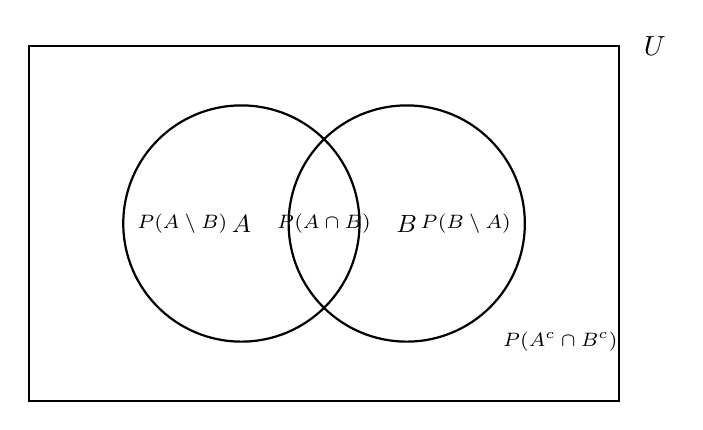
\begin{tikzpicture}[scale=1.5]
    % Draw universal set rectangle
    \draw[thick] (0,0) rectangle (5,3);
    \node at (5.3,3) {$U$};

    % Draw two overlapping circles
    \draw[thick] (1.8,1.5) circle (1);
    \draw[thick] (3.2,1.5) circle (1);

    % Labels for sets A and B
    \node at (1.8,1.5) [font=\small] {$A$};
    \node at (3.2,1.5) [font=\small] {$B$};

    % Probabilities in regions
    % A only region
    \node at (1.3,1.5) [font=\scriptsize] {$P(A \setminus B)$};
    % B only region
    \node at (3.7,1.5) [font=\scriptsize] {$P(B \setminus A)$};
    % Intersection region
    \node at (2.5,1.5) [font=\scriptsize] {$P(A \cap B)$};
    % Outside region
    \node at (4.5,0.5) [font=\scriptsize] {$P(A^c \cap B^c)$};
\end{tikzpicture}
\end{center}

\subsection*{Conditional Probability}
For events \( A, B \) with \( P(B) > 0 \):
\[
P(A \mid B) = \frac{P(A \cap B)}{P(B)}
\]

\subsection*{Multiplication Law}
\[
P(A \cap B) = P(A \mid B)P(B) = P(B \mid A)P(A)
\]

\subsection*{Law of Total Probability}
\[
P(A) = P(A \cap B) + P(A \cap B')
\]

\subsection*{Stated in terms of conditional probability}
\[
P(A \cap B) = P(A \mid B)P(B)
\]
\[
P(A \cap B') = P(A \mid B')P(B')
\]
\[
P(A) = P(A \mid B)P(B) + P(A \mid B')P(B')
\]

% Section: Random Variables and Distributions
\section*{Random Variables and Distributions}

\subsection*{Probability Mass Function (PMF)}
For a discrete random variable \( X \), the probability mass function \( P(X = x) \) is defined as:
\[
P(X = x) = \begin{cases}
  p_x & \text{if } x \in S, \\
  0 & \text{otherwise.}
\end{cases}
\]
\textbf{Definition:}
- \( X \): A discrete random variable.
- \( S \): The support (set of possible values that \( X \) can take).
- \( p_x \): The probability assigned to the outcome \( x \).

\subsection*{Bernoulli Distribution}
A random variable \( X \) follows a Bernoulli distribution if:
\[
P(X = x) = \begin{cases}
  p & \text{if } x = 1, \\
  1-p & \text{if } x = 0,
\end{cases}
\]
where \( p \in [0, 1] \) is the probability of success.

\textbf{Mean:} \( \mu = p \)

\textbf{Variance:} \( \sigma^2 = p(1-p) \)

\subsection*{Binomial Distribution}
A random variable \( X \) follows a Binomial distribution \( \text{Bin}(n, p) \) if it represents the number of successes in \( n \) independent Bernoulli trials:
\[
P(X = k) = \binom{n}{k} p^k (1-p)^{n-k}, \quad k = 0, 1, \dots, n.
\]
\textbf{Parameters:}
- \( n \): Number of trials.
- \( p \): Probability of success.

\textbf{Mean:} \( \mu = np \)

\textbf{Variance:} \( \sigma^2 = np(1-p) \)

\subsection*{Negative Binomial Distribution}
A random variable \( X \) follows a Negative Binomial distribution if it represents the number of trials required to achieve a fixed number of successes \( r \) in a sequence of independent Bernoulli trials with success probability \( p \):
\[
P(X = k) = \binom{k-1}{r-1} p^r (1-p)^{k-r}, \quad k = r, r+1, r+2, \dots
\]
\textbf{Parameters:}
- \( r \): Number of successes.
- \( p \): Probability of success in each trial.

\textbf{Mean:} \( \mu = \frac{r}{p} \)

\textbf{Variance:} \( \sigma^2 = \frac{r(1-p)}{p^2} \)

\textbf{Example:}
Suppose you are rolling a six-sided die, and you want to know the probability that the third "1" appears on the seventh roll. Here:
- \( r = 3 \) (three successes, rolling a "1").
- \( p = \frac{1}{6} \) (probability of rolling a "1" on a single trial).
- \( k = 7 \) (the total number of trials).

\[
P(X = 7) = \binom{6}{2}\left(\frac{1}{6}\right)^3\left(\frac{5}{6}\right)^4 \approx 0.0335
\]

\textbf{Real-World Application}
The Negative Binomial distribution is commonly used to model scenarios where we are counting the number of trials needed to achieve a fixed number of successes. For example:
- In customer service, modeling the number of calls needed to resolve \( r \) issues when the probability of resolving an issue in a single call is \( p \).
- In biology, determining the number of experiments required to observe \( r \) successful outcomes of a rare event.

\subsection*{Poisson Distribution}
A random variable \( X \) follows a Poisson distribution \( \text{Poisson}(\lambda) \) if it represents the number of events occurring in a fixed interval:
\[
P(X = k) = \frac{\lambda^k e^{-\lambda}}{k!}, \quad k = 0, 1, 2, \dots
\]
\textbf{Parameter:}
- \( \lambda \): Average rate of occurrence.

\textbf{Mean:} \( \mu = \lambda \)

\textbf{Variance:} \( \sigma^2 = \lambda \)

\subsection*{Geometric Distribution}
A random variable \( X \) follows a Geometric distribution if it represents the trial count until the first success in a series of independent Bernoulli trials with success probability \( p \):
\[
P(X = k) = (1 - p)^{k - 1}p, \quad k = 1, 2, 3, \dots
\]
\textbf{Parameters:}
\begin{itemize}
    \item \( p \): Probability of success on each trial.
\end{itemize}

\textbf{Mean:} \( \mu = \frac{1}{p} \)

\textbf{Variance:} \( \sigma^2 = \frac{1 - p}{p^2} \)

\textbf{Standard Deviation:} \( \sigma = \sqrt{\frac{1 - p}{p^2}} \)

\textbf{When to Use:}
Geometric distributions model the number of trials until the first success, common in reliability testing, queue theory, and repeated experiments until success.

\subsection*{Gaussian (Normal) Distribution}
A random variable \( X \) follows a Gaussian distribution \( \mathcal{N}(\mu, \sigma^2) \) if its probability density function (PDF) is:
\[
P(X = x) = \frac{1}{\sqrt{2\pi\sigma^2}} \exp\left(-\frac{(x-\mu)^2}{2\sigma^2}\right).
\]
\textbf{Parameters:}
- \( \mu \): Mean (center of the distribution).
- \( \sigma^2 \): Variance (spread of the distribution).

\textbf{Properties:}
- Symmetric about \( \mu \).
- \( X \sim \mathcal{N}(\mu, \sigma^2) \) satisfies the Empirical Rule:
  - 68\% of data within \( [\mu - \sigma, \mu + \sigma] \).
  - 95\% of data within \( [\mu - 2\sigma, \mu + 2\sigma] \).
  - 99.7\% of data within \( [\mu - 3\sigma, \mu + 3\sigma] \).

\section*{Expected Value and Variance}

\subsection*{Expected Value}
For a discrete random variable \( X \) with possible values \( x_1, x_2, \dots, x_n \) and corresponding probabilities \( P(X = x_i) \):
\[
E[X] = \sum_{i=1}^n x_i P(X = x_i)
\]

\textbf{Example:}
If \( X \) has the following probability mass function (PMF):
\begin{center}
\begin{tabular}{|c|c|}
\hline
\( x \) & \( P(X = x) \) \\
\hline
1 & 0.2 \\
2 & 0.5 \\
3 & 0.3 \\
\hline
\end{tabular}
\end{center}
The expected value is:
\[
E[X] = (1 \times 0.2) + (2 \times 0.5) + (3 \times 0.3) = 2.1
\]

\subsection*{Generalized Extreme Value (GEV) Distribution}
A random variable \(X\) follows a GEV distribution if it models the maxima or minima of samples of various distributions:
\[
f_X(x; \mu, \sigma, \xi) = \frac{1}{\sigma} \left[1 + \xi \left(\frac{x - \mu}{\sigma}\right)\right]^{-\frac{1}{\xi} - 1} \exp\left(-\left[1 + \xi \frac{x - \mu}{\sigma}\right]^{-\frac{1}{\xi}}\right),
\]
where \(\xi \neq 0\), \(\sigma > 0\), and the domain of \(x\) depends on \(\xi\).

\textbf{Parameters:}
- Location: \(\mu\)
- Scale: \(\sigma\)
- Shape: \(\xi\)

\textbf{Mean (\(\xi < 1\)):}
\[
\mu + \frac{\sigma}{\xi}(\Gamma(1-\xi) - 1)
\]

\textbf{Variance:}
\[
\frac{\sigma^2}{\xi^2}[\Gamma(1 - 2\xi) - \Gamma^2(1 - \xi)], \quad \xi < 0.5
\]

\textbf{Standard Deviation:} Square root of variance.

\textbf{Applications:}
- Extreme environmental events (floods, earthquakes).
- Financial risk management.

\subsection*{Solving for the Mean of a Normal Distribution Using Symmetry}

Given a normal random variable \( X \sim N(\mu, 2^2) \), and the probability:
\[
P(-4\mu < X < 6\mu) = 0.6528
\]
we are asked to solve for the mean \( \mu \).

\textbf{Step-by-Step Calculation:}

1. Recognize the interval is symmetric about \( \mu \):

\quad\quad\( 6\mu - \mu = \mu - (-4\mu) = 5\mu \).

2. Express the interval in terms of deviation from the mean:

\quad\quad\( P(\mu - 5\mu < X < \mu + 5\mu) \).

3. Rewrite as: \( P(-5\mu < X - \mu < 5\mu) \).

4. Standardize using \( Z = \frac{X - \mu}{2} \).

5. The probability becomes: \( P\left( \frac{-5\mu}{2} < Z < \frac{5\mu}{2} \right) \).

6. Use symmetry: \( P\left( 0 < Z < \frac{5\mu}{2} \right) = \frac{0.6528}{2} = 0.3264 \).

7. Total cumulative area: \( \Phi\left( \frac{5\mu}{2} \right) = 0.5 + 0.3264 = 0.8264 \).

8. Invert the standard normal CDF: \( \Phi^{-1}(0.8264) = 0.94 \).

9. Set up equation: \( \frac{5\mu}{2} = 0.94 \).

10. Solve for \( \mu \): \( \mu = \frac{2 \cdot 0.94}{5} = 0.376 \).

11. Round to two decimal places: \( \mu \approx 0.38 \).


\subsection*{Variance of a Random Variable}
The variance of a random variable \( X \) measures the spread of its values around the mean \( \mu = E[X] \):
\[
\text{Var}(X) = E[(X - \mu)^2] = E[X^2] - (E[X])^2
\]
\textbf{Step-by-Step Calculation:}
1. Compute \( E[X] \).
2. Compute \( E[X^2] = \sum_{i=1}^n x_i^2 P(X = x_i) \).
3. Subtract \( (E[X])^2 \) from \( E[X^2] \).

\textbf{Example:}
Using the PMF from above:
\[
E[X^2] = (1^2 \times 0.2) + (2^2 \times 0.5) + (3^2 \times 0.3) = 0.2 + 2.0 + 2.7 = 4.9
\]
\[
\text{Var}(X) = E[X^2] - (E[X])^2 = 4.9 - (2.1)^2 = 4.9 - 4.41 = 0.49
\]

\subsection*{Properties of Expected Value and Variance}
- For a constant \( c \):
\[
E[c] = c, \quad \text{Var}(c) = 0
\]
- For a random variable \( X \):
\[
E[cX] = cE[X], \quad \text{Var}(cX) = c^2\text{Var}(X)
\]
- For independent random variables \( X \) and \( Y \):
\[
\text{Var}(X + Y) = \text{Var}(X) + \text{Var}(Y)
\]

\subsection*{Application: Linear Combinations of Random Variables}
For \( Y = aX + b \):
\[
E[Y] = aE[X] + b, \quad \text{Var}(Y) = a^2\text{Var}(X)
\]

% Second Section: Statistics
\section*{Statistics}

\subsection*{Variance and Covariance}
For a random variable \(X\) with mean \(\mu_X = E[X]\):

\[
\text{Var}(X) = E[(X - \mu_X)^2] = E[X^2] - (E[X])^2
\]

For two random variables \(X\) and \(Y\) with means \(\mu_X, \mu_Y\):
\[
\text{Cov}(X,Y) = E[(X - \mu_X)(Y - \mu_Y)] = E[XY] - E[X]E[Y]
\]

Sample-based formulas for \(n\) data points \((x_i, y_i)\):
\[
\bar{x} = \frac{1}{n}\sum_{i=1}^n x_i, \quad \bar{y} = \frac{1}{n}\sum_{i=1}^n y_i
\]

\[
s_X^2 = \frac{1}{n-1}\sum_{i=1}^n (x_i - \bar{x})^2, \quad
s_Y^2 = \frac{1}{n-1}\sum_{i=1}^n (y_i - \bar{y})^2
\]

\[
\text{Cov}(X,Y) = \frac{1}{n-1}\sum_{i=1}^n (x_i - \bar{x})(y_i - \bar{y})
\]

\subsection*{Linear Regression}
For a simple linear regression with one predictor \( X \) and response \( Y \), the model is:
\[
Y = \beta_0 + \beta_1 X + \varepsilon
\]

The least-squares estimates for \(\beta_0\) and \(\beta_1\) using \(n\) observations \((x_i, y_i)\) are:
\[
\hat{\beta}_1 = \frac{\sum_{i=1}^n (x_i - \bar{x})(y_i - \bar{y})}{\sum_{i=1}^n (x_i - \bar{x})^2} = \frac{\text{Cov}(X,Y)}{s_X^2}
\]

\[
\hat{\beta}_0 = \bar{y} - \hat{\beta}_1 \bar{x}
\]

The fitted line is:
\[
\hat{Y} = \hat{\beta}_0 + \hat{\beta}_1 X
\]

% Third Section: Combinatorics
\section*{Combinatorics}

\subsection*{Factorials}
For a positive integer \(n\):
\[
n! = n \times (n-1) \times (n-2) \times \cdots \times 2 \times 1
\]
By definition, \(0! = 1\}.

\subsection*{Permutations}
The number of ways to arrange \(k\) distinct objects out of \(n\) distinct objects (order matters):
\[
P(n, k) = \frac{n!}{(n-k)!}
\]

\subsection*{Combinations}
The number of ways to choose \(k\) elements out of \(n\) without regard to order (also called \(\binom{n}{k}\)):
\[
C(n, k) = \binom{n}{k} = \frac{n!}{k!(n-k)!}
\]

Common notation:
- Combinations: \(\binom{n}{k}\), \(C(n,k)\)
- Permutations: \(P(n,k)\) or sometimes \(_nP_k\)

\subsection*{Examples}
\[
\binom{5}{2} = \frac{5!}{2! \cdot 3!} = \frac{120}{2 \cdot 6} = 10
\]

\[
P(5,2) = \frac{5!}{(5-2)!} = \frac{5!}{3!} = \frac{120}{6} = 20
\]

\end{multicols}

\end{document}
